\documentclass{beamer}
\usepackage{hyperref}
\usetheme{Madrid}
\title{Coarse graining molecular dynamics with graph neural networks}
\author{Andrew Bruce\inst{1}}
\institute[UCSC] {
  \inst{1}
  University Of California, Santa Cruz
}
\date{2024-10-24}
\begin{document}
\frame{\titlepage}
\begin{frame}
  \frametitle{Problem}
  \href{https://arxiv.org/abs/1706.08566}{First paper link}
  \begin{block}{Why}
    Evaluating the forces on atoms in a protein is very computationally expensive.
  \end{block}
  Create some ``model'' that takes in $n$ atom types $\mathbf{Z} = ( Z_1, \dots, Z_n)$ and positions $\mathbf{R} = ( \vec{r}_1, \dots, \vec{r}_n )$, where $ \vec{r}_i \in \mathbb{R}^3$ and tries to calculate the forces $\mathbf{\hat{F}}(\mathbf{R}, \mathbf{Z}) = ( \vec{f}_1, \dots, \vec{f}_n )$ on each atom. It should be \alert{invariant} over translations and rotations. The force field should preserve the conservation of energy. The model should also be able to take in \alert{any number} of atoms.
\end{frame}
\begin{frame}
  \frametitle{Enforcing Invariants}
  \begin{block}{Rotations and translations}
    Make the model only use the distances between atoms, \alert{NOT} their absolute cartesian coordinates.
  \end{block}
  The model should only depend on $\| \vec{r}_i - \vec{r}_j \|$ between any two atoms, but \alert{never} $\vec{r}_i$ alone.
\end{frame}
\begin{frame}
  \frametitle{Enforcing Invariants}
  \begin{block}{Conservation of energy}
    Instead of the model calculating the forces $\mathbf{\hat{F}}(\mathbf{R}, \mathbf{Z}) \in \mathbb{R}^{3 \times n}$, calculate the energy $E(\mathbf{R}, \mathbf{Z}) \in \mathbb{R}$, then take the \alert{gradient with respect to the positions} to calculate the force.
    $\mathbf{\hat{F}} = \nabla_{\mathbf{R}} E$
  \end{block}
  Any force field like this is now impossible: 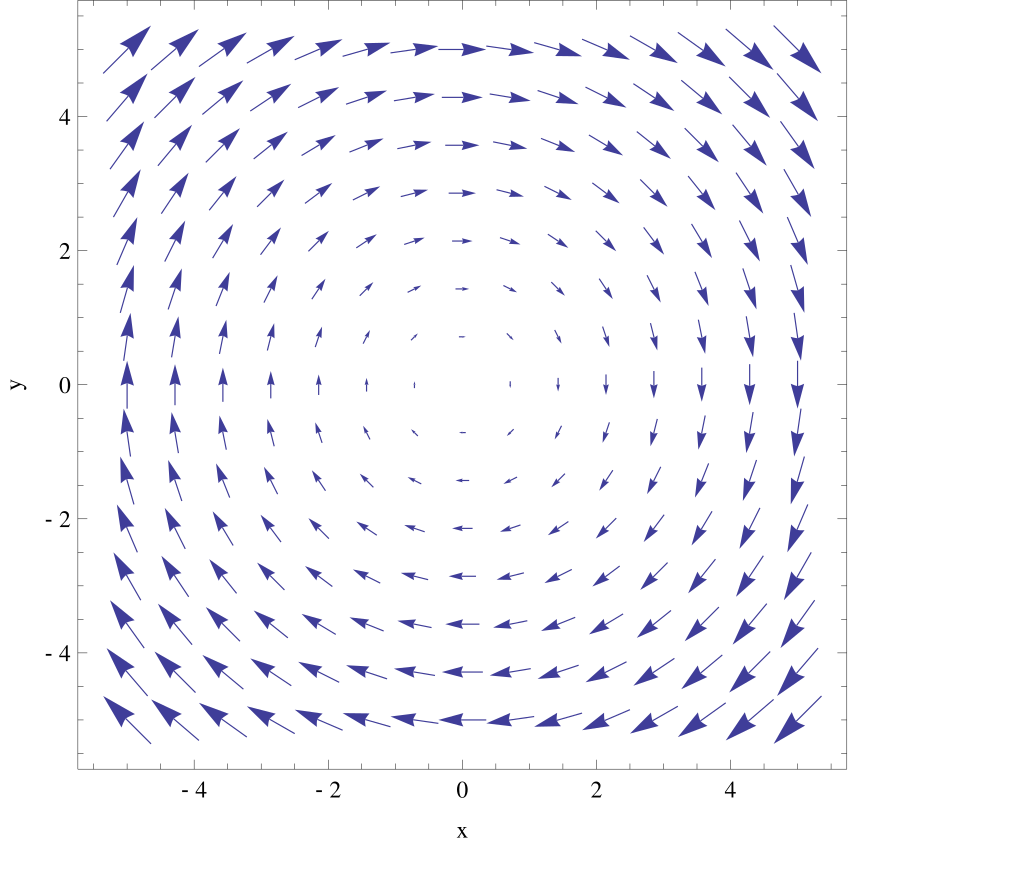
\includegraphics[width=0.35\linewidth]{./curl.png}
\end{frame}
\begin{frame}
  \frametitle{Schnet Architecture}
  \begin{center}
    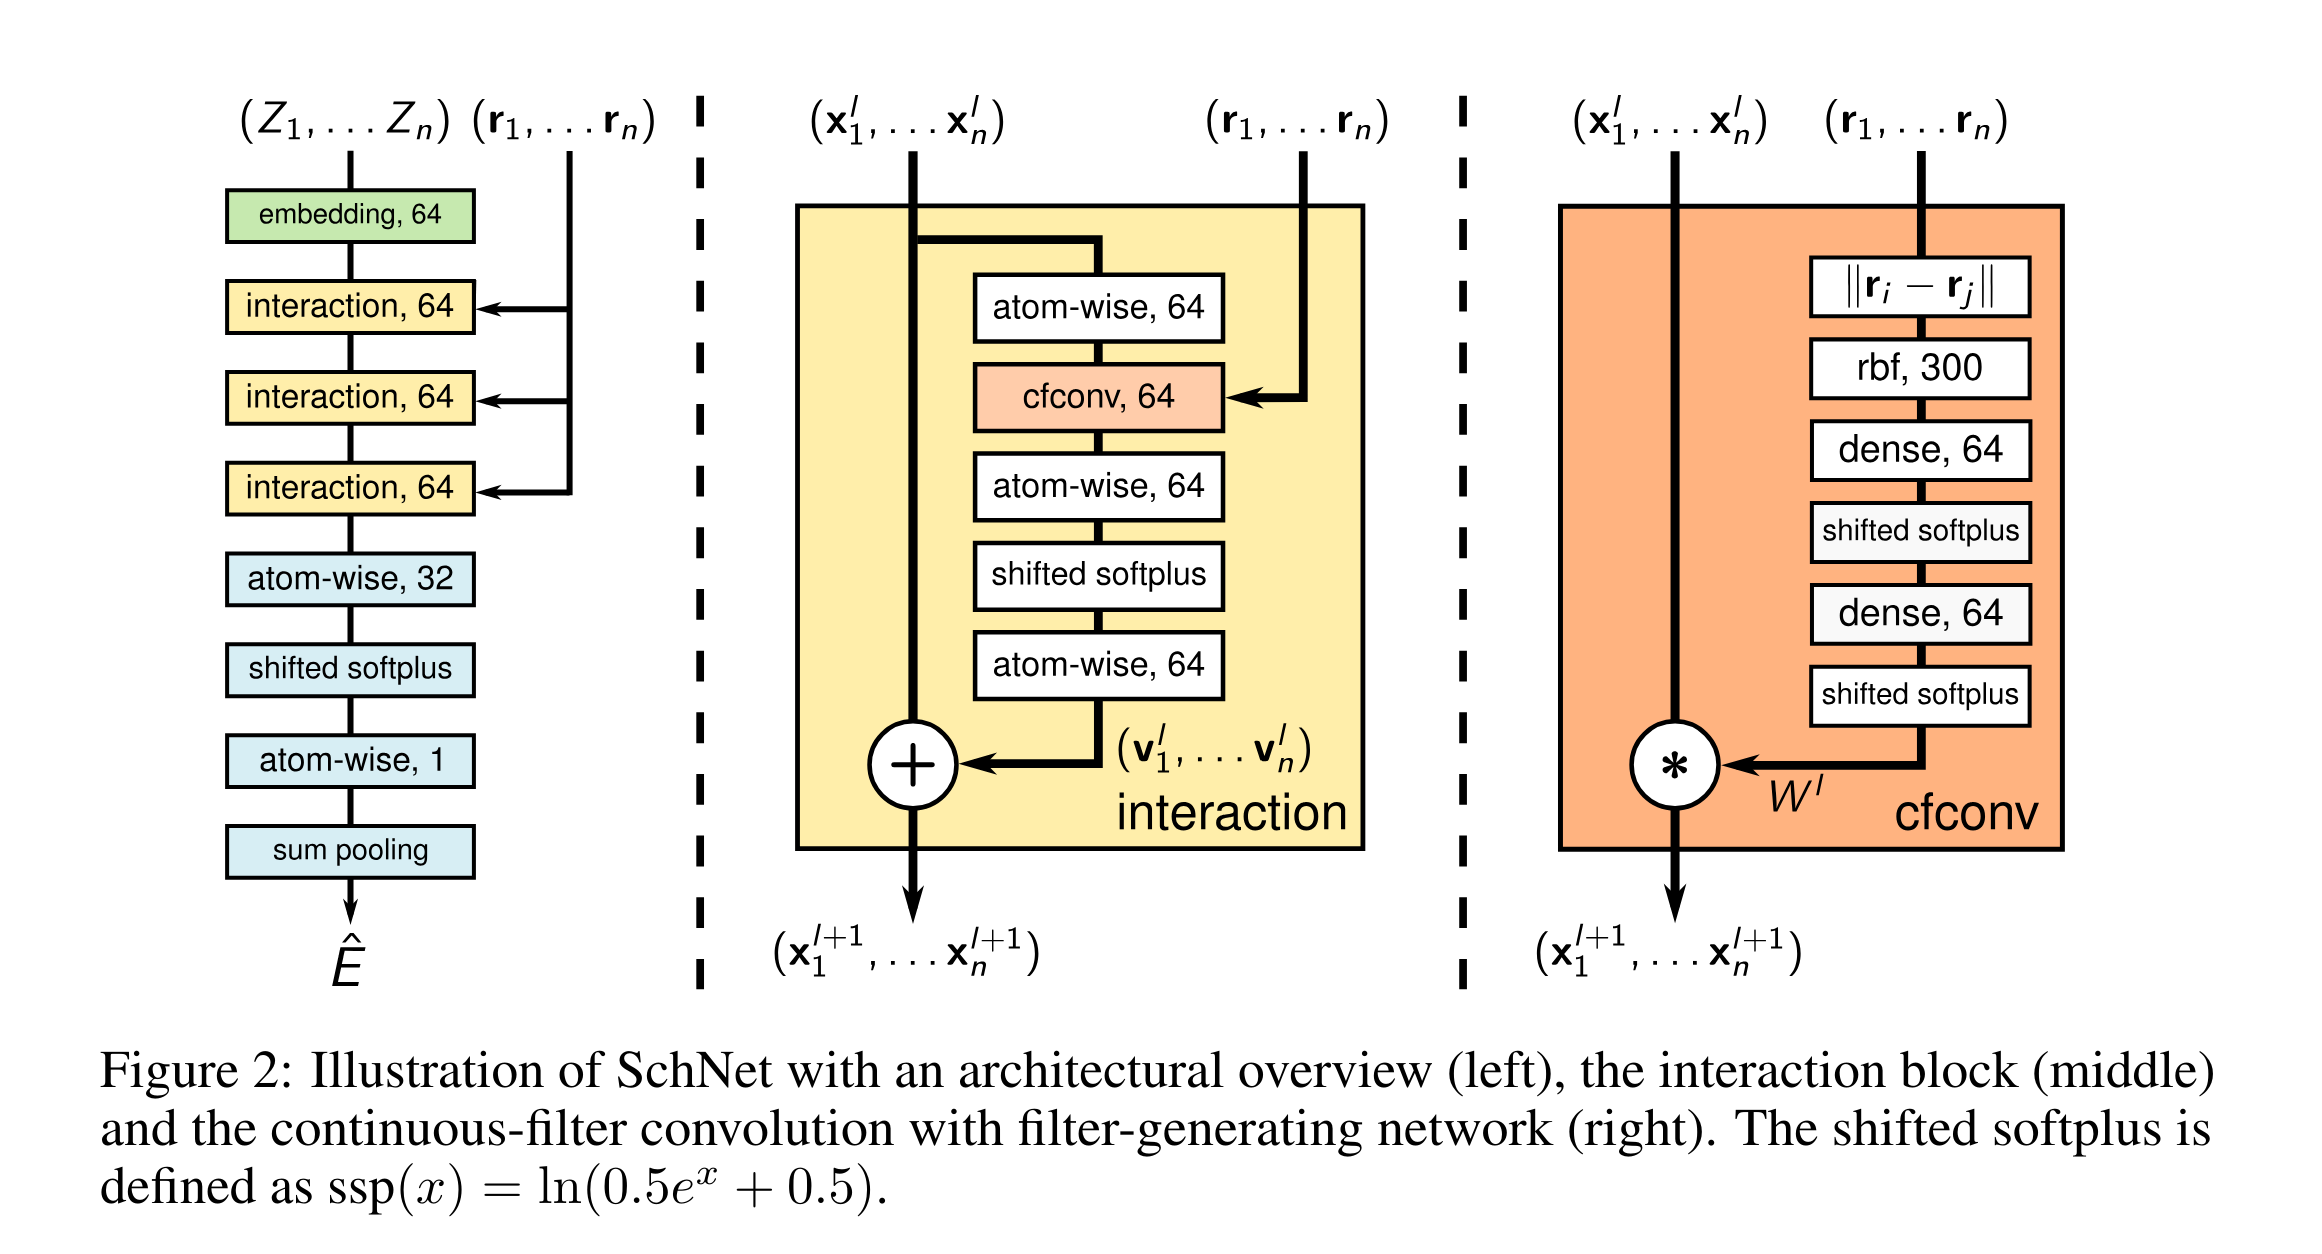
\includegraphics[width=0.5\linewidth]{./archetecture_overview.png}
  \end{center}
  The input embeddings are based off the atom type, $\vec{x}^0_i = a_{Z_i}$.
  \begin{block}{Atom wise layers}
    For each atom wise layer The parameters $W$ an $b$ are applied to the features of each atom $i$.
    $$\vec{x}_i^{l+1} = W\vec{x}_i^l + b$$
  \end{block}
\end{frame}
\begin{frame}
  \frametitle{Continuous-filter convolutions}
  \begin{minipage}{4cm}
    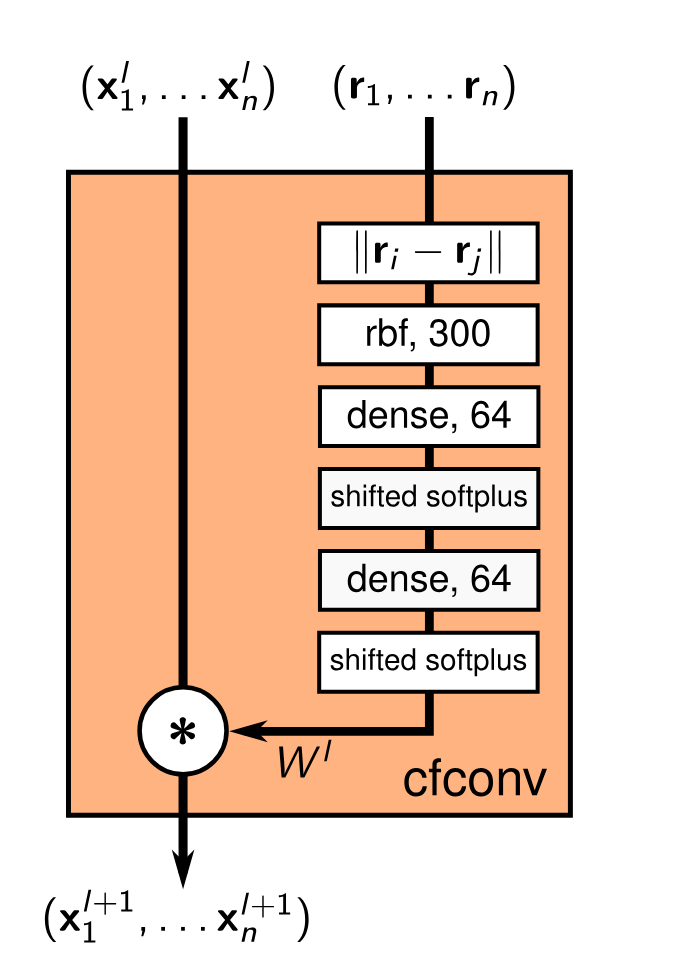
\includegraphics[width=\linewidth]{./cfconv_block.png}
  \end{minipage}% needs this comment for linebreak or something?
  \small\begin{minipage}{8cm}
  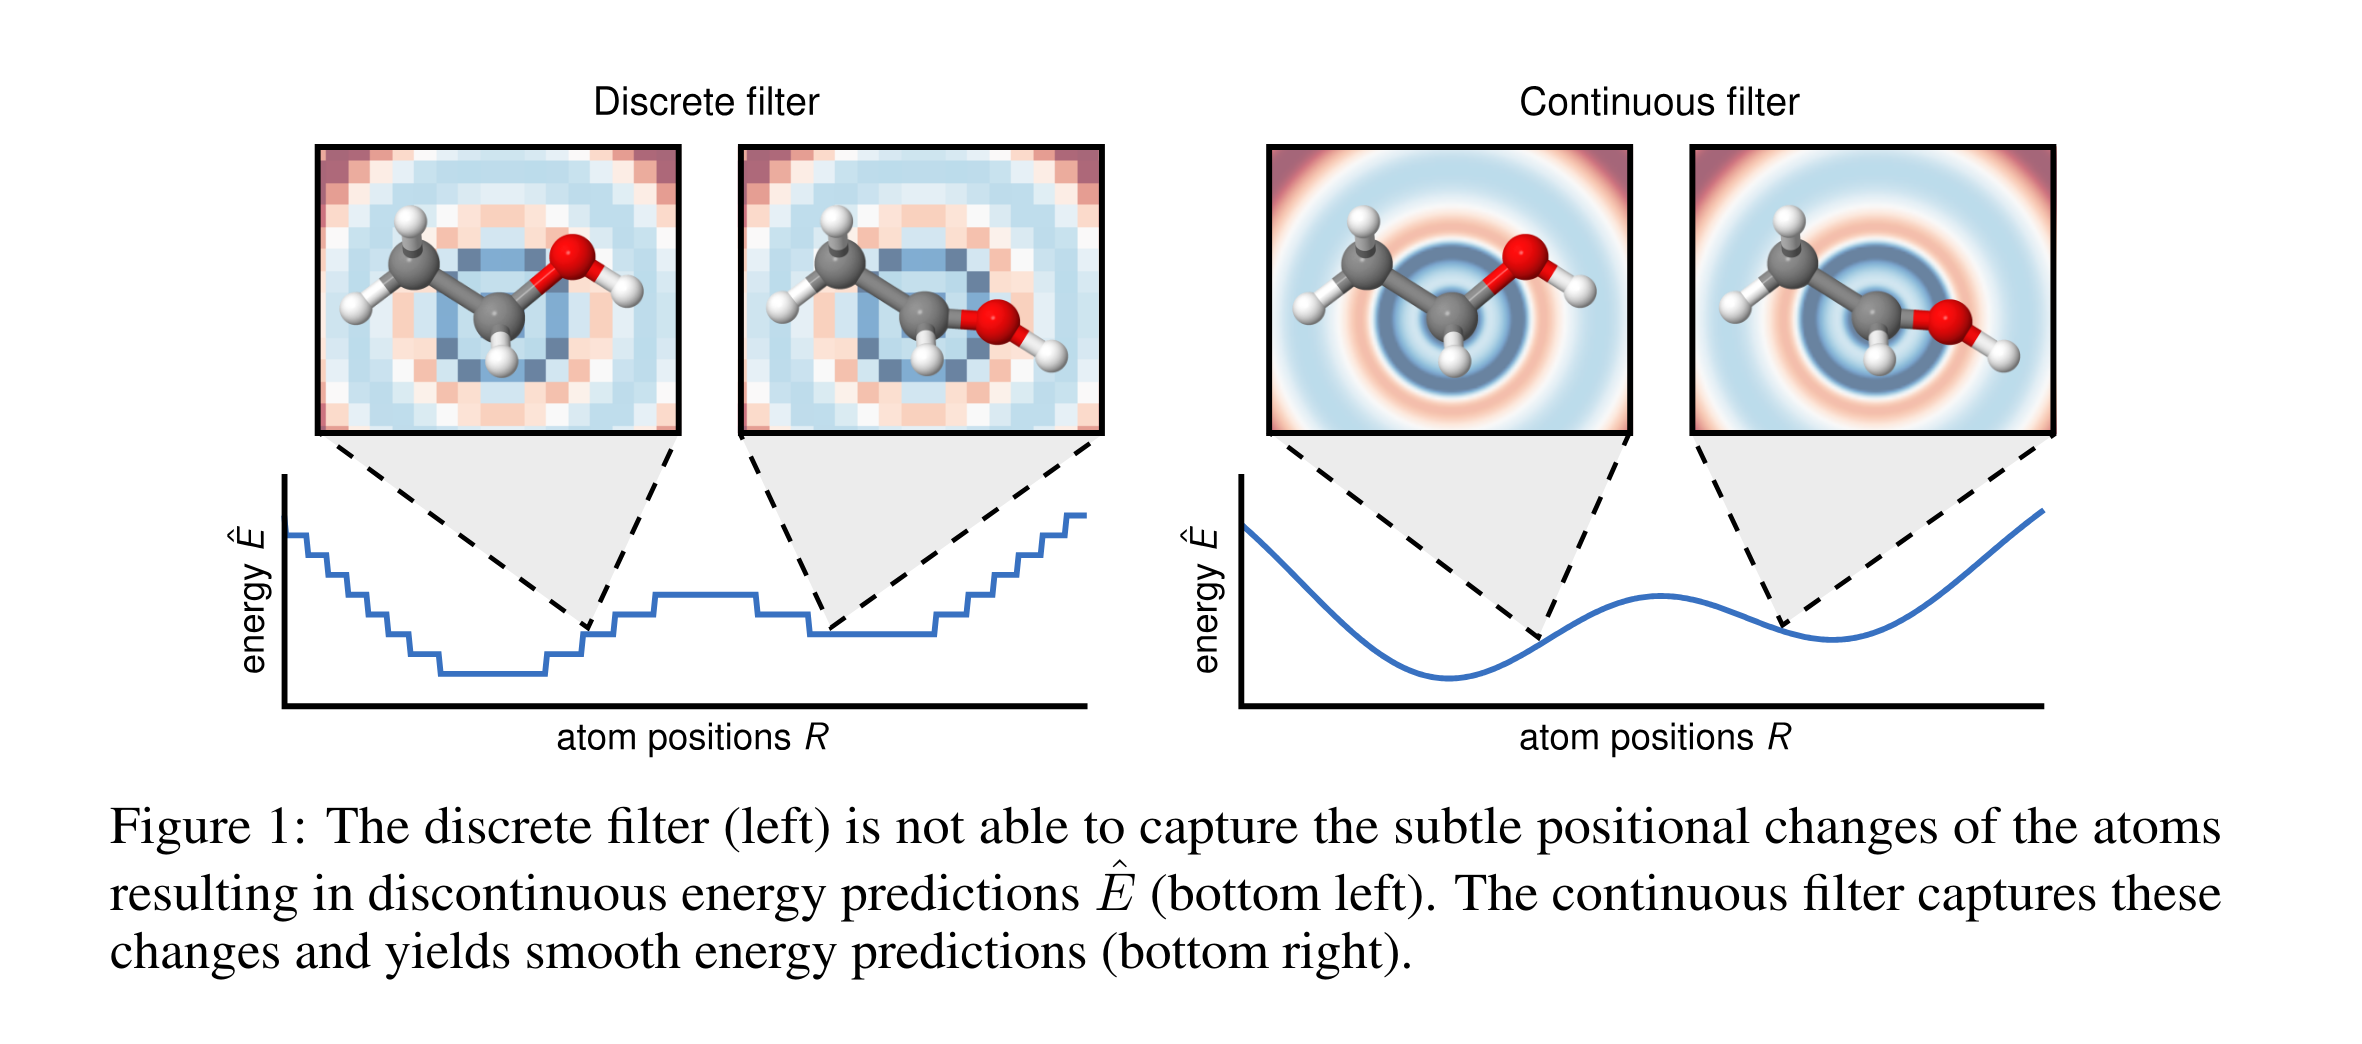
\includegraphics[width=\linewidth]{./cfconv.png}
  Attempt continious convolutions for unevenly spaced points.
  Learn some filter function $W$, and for each atom $i$ the next feature is $\vec{x}_i^{l+1} = \sum_j \vec{x}_j^l \circ W(\vec{r}_i - \vec{r}_j)$, where $\circ$ is element wise multiplication.
  \end{minipage}
  \begin{block}{Radial basis function}
    The radial basis functions will create a vector $\vec{e}$ where each element $\vec{e}_k(\vec{r}_i - \vec{r}_j) = e^{-\gamma (||r_i - r_j|| - \mu_k)^2}$.
  \end{block}
\end{frame}
\begin{frame}
  \frametitle{Training}
  The loss function is a combined energy and force loss. The output of the model $M$ is just one scalar, the energy $E = M(\mathbf{Z}, \mathbf{R})$. Given the training data consisting of the real energy $E^{real}$ and forces $F^{real}$.
  \begin{center}
    $L(M, \mathbf{Z}, \mathbf{R}) = \text{energy error} + \text{force error}$\\
    $= \rho(M(\mathbf{Z}, \mathbf{R}) - E^{real})^2 + \dfrac{1}{n} \| F^{real} - \nabla_{\mathbf{R}}M(\mathbf{Z}, \mathbf{R}) \|^2$\\
    $= \rho(E - E^{real})^2 + \dfrac{1}{n} \sum^n_{i=1} \sum^3_{d=1} ( F^{real}_{i_d} - \dfrac{\partial E}{\partial r_{i_d}} )^2$
  \end{center}
  \begin{block}{Double differentiation? Double backpropigation?}
    Gradient descent with respect to the weights $\mathbf{W}$ is:
    \begin{center}
      $\mathbf{W}_{t+1} = \mathbf{W}_t - \lambda \nabla_{\mathbf{W}} L(W)$
    \end{center}
    The entire network must be double differentiable...
  \end{block}
\end{frame}
\begin{frame}
  \frametitle{Results}
  Not that good ... but the invention of the continious-filter convolution will be useful in the next paper.
  \begin{center}
    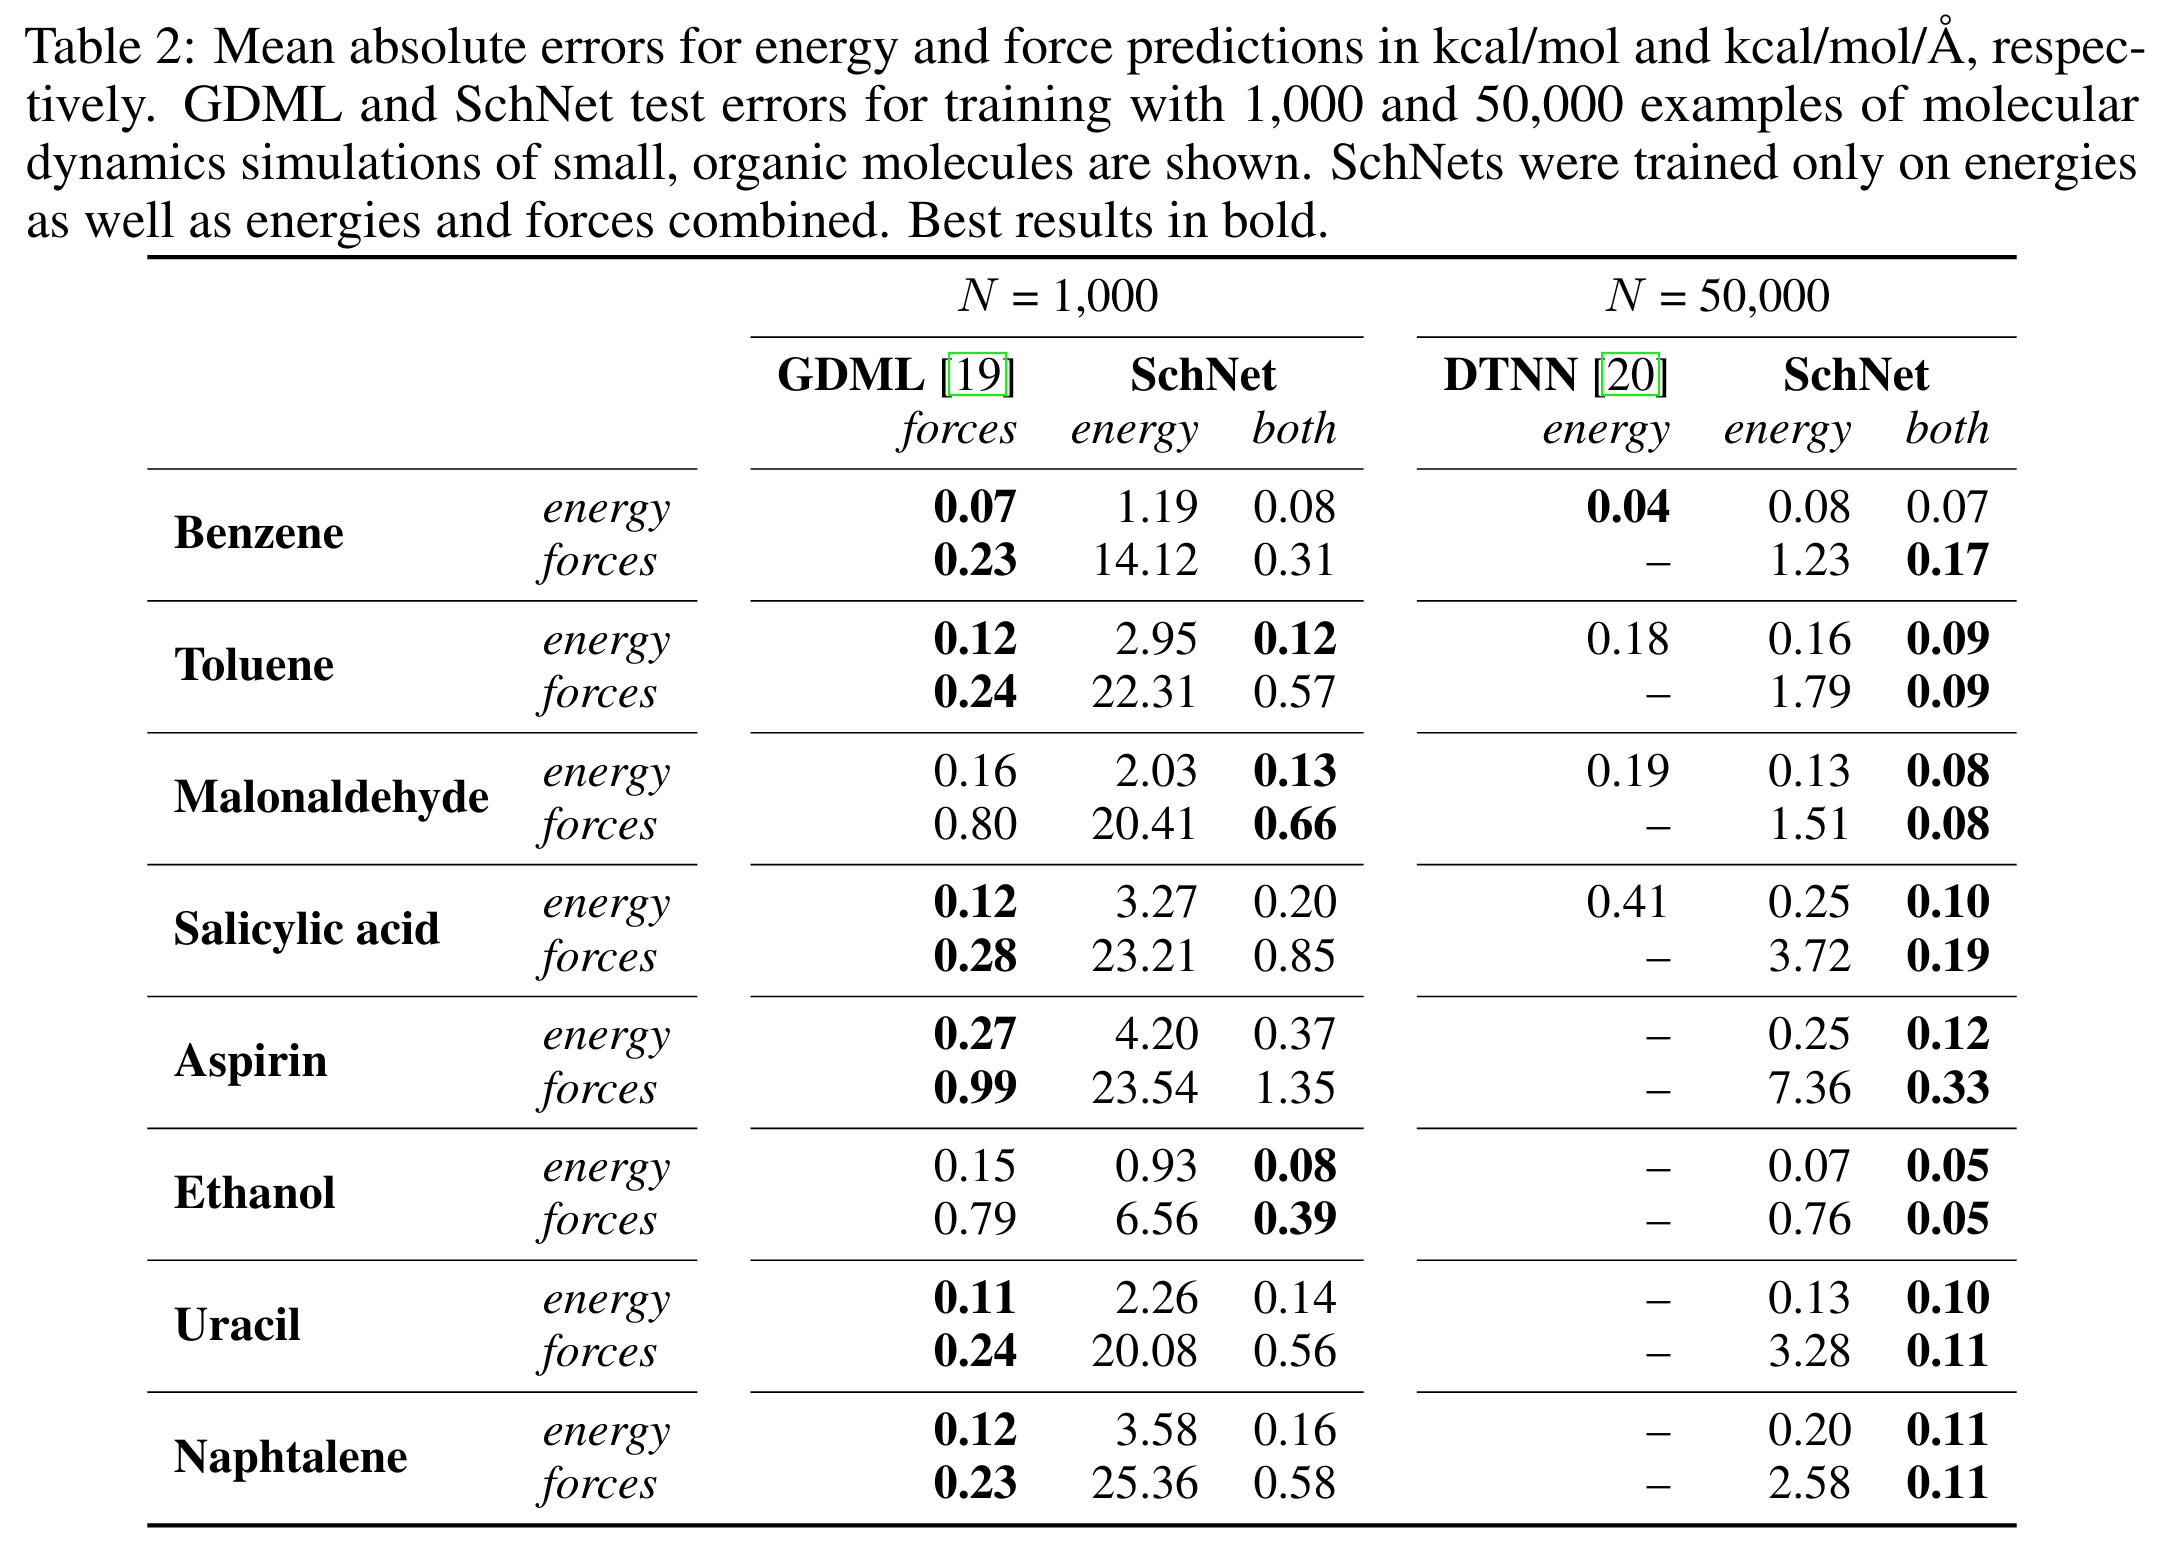
\includegraphics[width=0.7\linewidth]{./paper1_results.png}
  \end{center}
\end{frame}
\begin{frame}
  \frametitle{Paper 2}
  \huge \href{https://arxiv.org/abs/2007.11412}{Next paper link}\\
  \huge Schnet + CGnet = CGSchnet
\end{frame}
\begin{frame}
  \frametitle{Coarse graining}
  We want to map $n$ atoms to $N$ ``interaction sites''. We use a matrix $\Xi$ to map $\mathbb{R}^{3n} \longrightarrow \mathbb{R}^{3N}$. Given $r \in \mathbb{R}^{3n}$, the coarse grained $R = \Xi r$. In this paper $\Xi$ only consists of ones and zeros, so only a subset of the atom positions are used, and the rest of the information is discarded.
  \begin{center}
    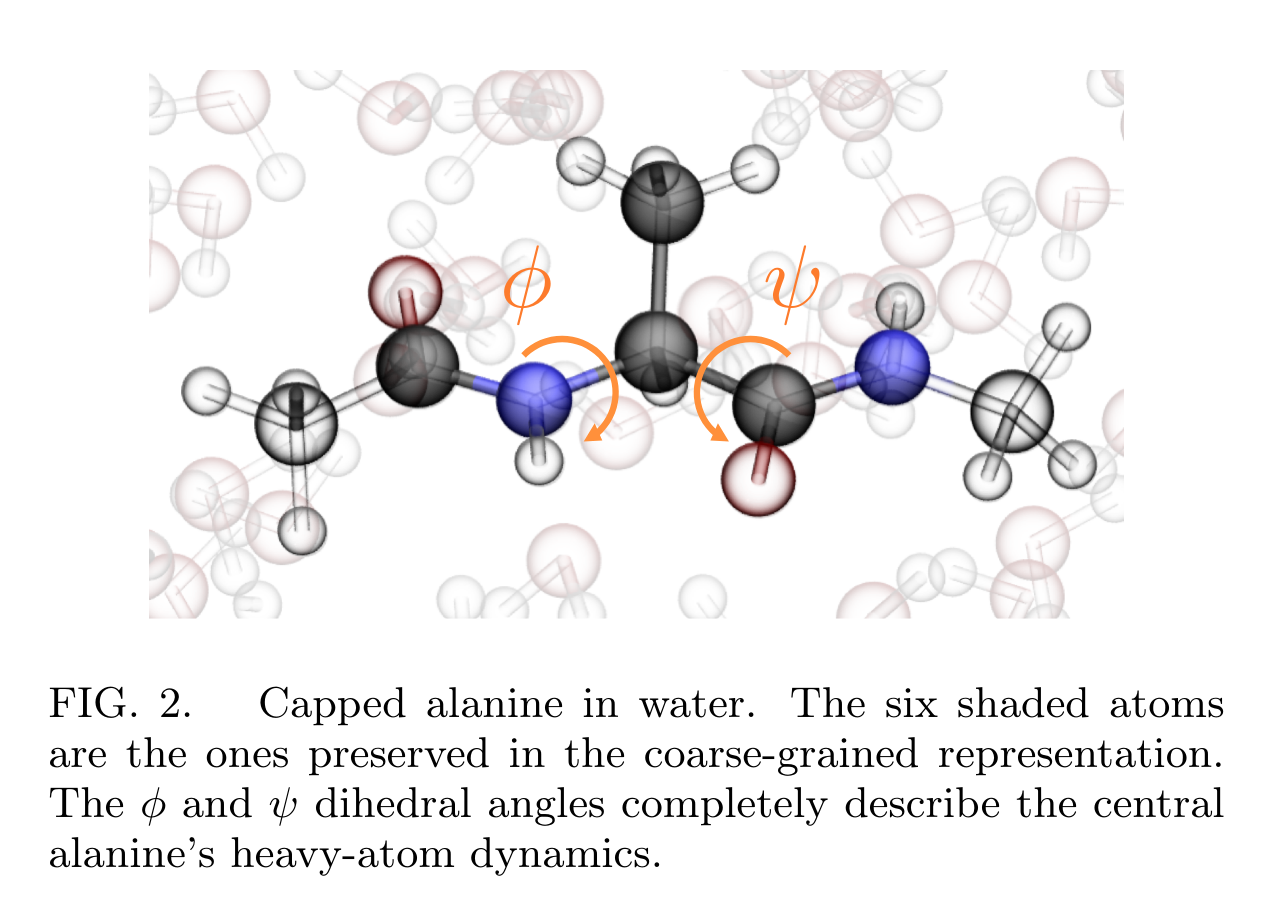
\includegraphics[width=0.7\linewidth]{./coarse_graining.png}
  \end{center}
\end{frame}
\begin{frame}
  \frametitle{Quick Tangent, Graph Neural Networks}
  Dense layers map features to features
  \begin{center}
    $F^A \longrightarrow F^B$
  \end{center}
  Convolutional layers map a $n$ dimenstional grid of features $F_{in}$ to a grid by applying a convoltution with a kernel function $\phi \in  \mathbf{R}^n \longrightarrow \mathbf{R}$.
  \begin{center}
    $F_{in}^{A_1 \times \dots \times A_n} \longrightarrow F_{out}^{B_1 \times \dots \times B_n}$
  \end{center}
  Graph layers maps graphs to graphs using a graph convolution functions $\psi_v \in (V, G) \longrightarrow F$, $\psi_e \in (E, G) \longrightarrow F_{e, out}$
  \begin{center}
    $(V_{F_{v, in}}, E_{F_{e, in}}) \longrightarrow (V_{F_{v, out}}, E_{F_{e, out}})$
  \end{center}
  The graphs can have any number of verticies or edges.
\end{frame}
\begin{frame}
  \frametitle{GNNs: Arbitrary structure}
  GNN's allow arbitrary structure of data to be passed in.
  \begin{block}{Invariance over graph permutations}
    For example the output features of a vector $v \in V$ with a set of connected edges $N_v$ could look like:
    \begin{center}
      $\phi(f_v, \oplus_{u \in N_v}\psi(f_v, f_u, f_{e_{uv}}))$
    \end{center}
    Where $f_v$ or $f_e$ is the feature for the coresponding vertex or edge. $\oplus$ should be a permutation-invariant aggregator to preserve the networks invariance.
  \end{block}
  Because it is invariant over permutations of the verticies, and we can structure the graph however we want we don't require every atom to be interacting with every other.
\end{frame}
\begin{frame}
  \frametitle{GNNs: Arbitrary structure}
  \begin{minipage}{6cm}
    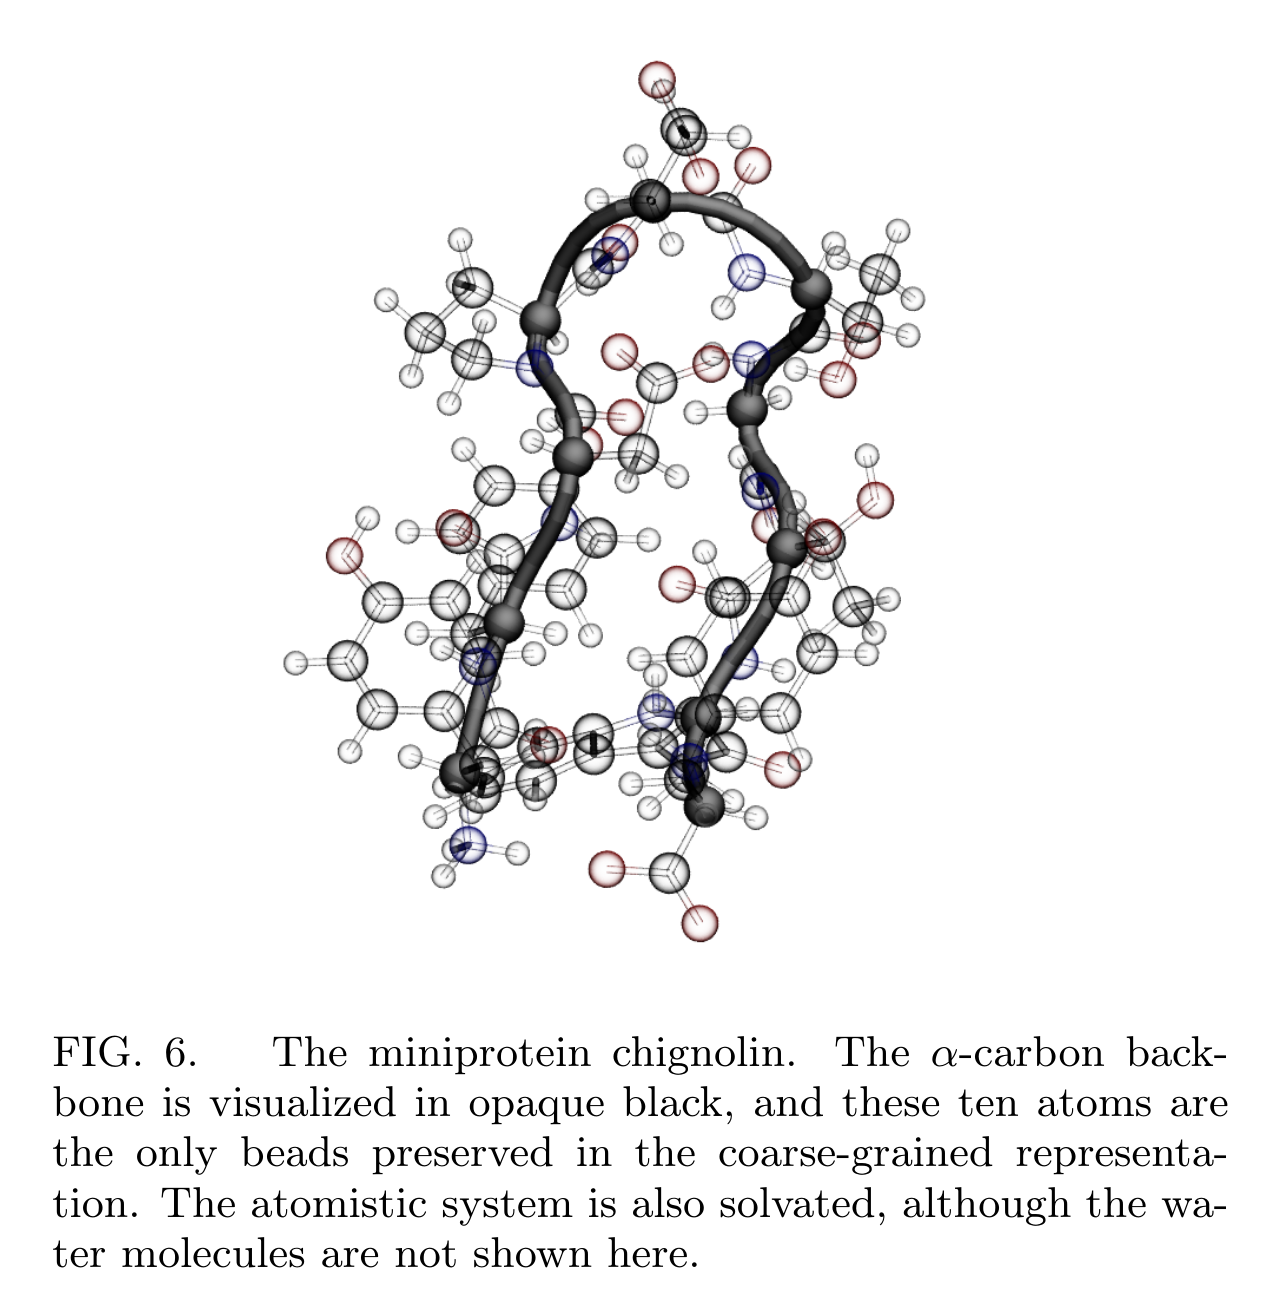
\includegraphics[width=\linewidth]{./coarse_graining2.png}
  \end{minipage}% aa
  \begin{minipage}{6cm}
    Not all atoms must have edges between them. For each frame at positions $R$, edges can only be added if interaction sites are smaller than some distance $\epsilon$. Fewer edges requires less calculations in the graph neural network.
  \end{minipage}
\end{frame}
\begin{frame}
  \frametitle{CGSchnet Archetecture}
  \begin{center}
    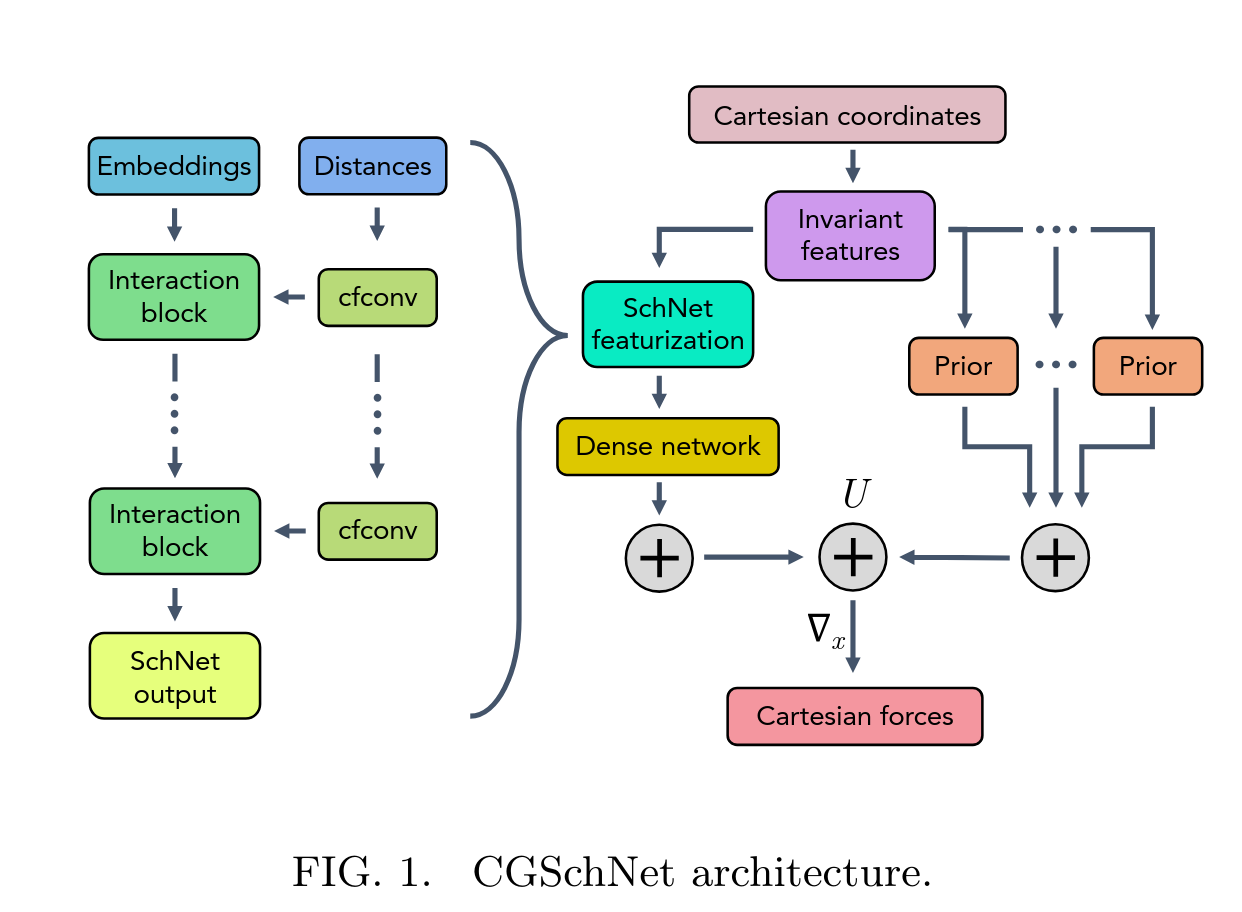
\includegraphics[width=0.5\linewidth]{./cgschnet_arch.png}
  \end{center}
  Create a network similar to Schnet with ``cfconf'' as the graph convolutions, but with the addition of coarse graining and adding a ``prior'' that acts as a bad simulation extimated from the training data of a protein. Many different priors to choose from, usually estimates bonds as spring constants with some harmonic motion.
\end{frame}
\begin{frame}
  \frametitle{Prior}
  \begin{center}
    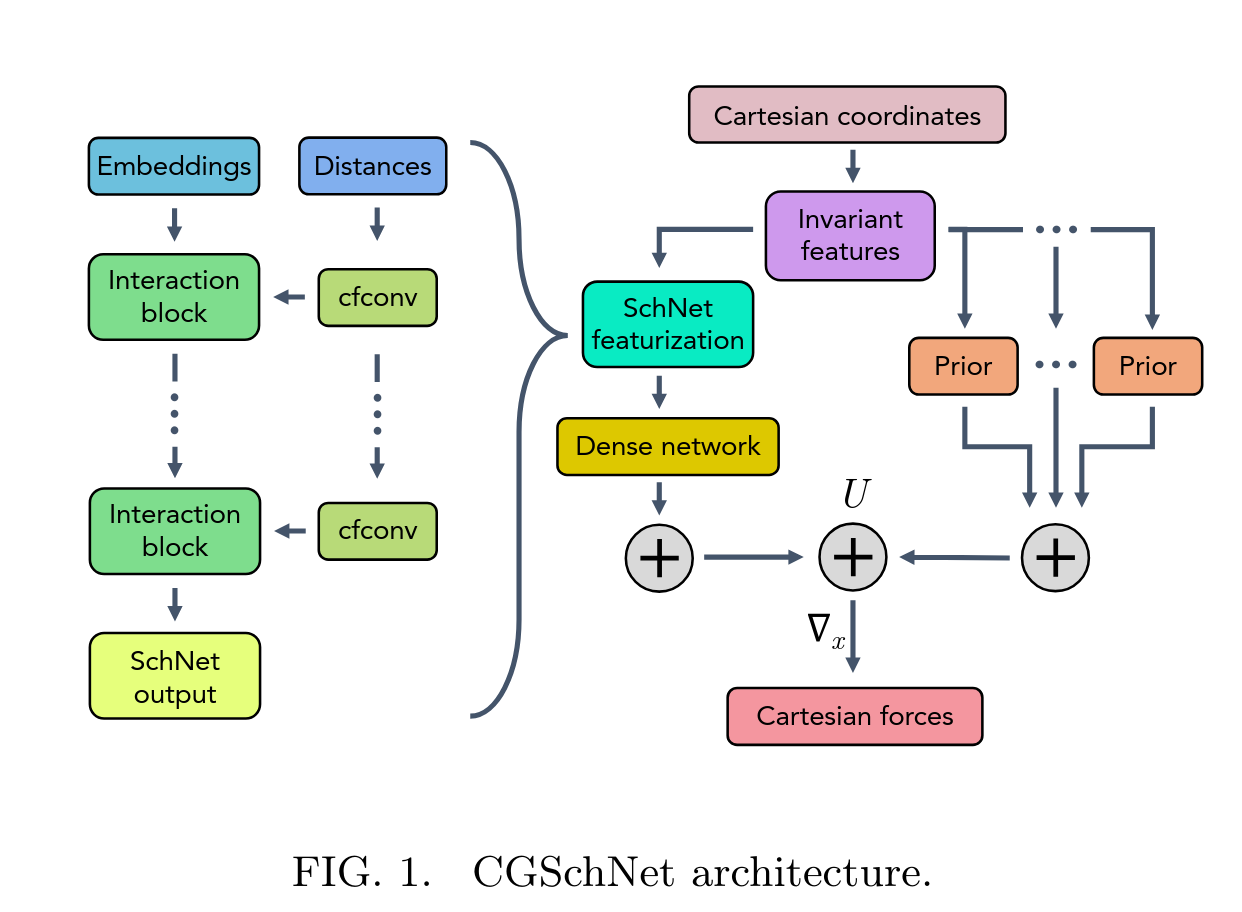
\includegraphics[width=0.3\linewidth]{./cgschnet_arch.png}
  \end{center}
  \small\begin{block}{Why is it called the ``prior''?}
  MLE for Bayesian inference has an equation given a model $\theta$ and data $D$:\\
  \begin{center}
    $\text{posterior} = P(\theta | D) = \dfrac{P(D | \theta) P(\theta)}{P(D)} = \dfrac{\text{likelyhood} \times \text{prior}}{\text{marginal}}$
  \end{center}
  If $P(D)$ is constant then
  \begin{center}
    $\ln(P(D | \theta) P(\theta)) = \ln(P(D | \theta)) + \ln(P(\theta))$
  \end{center}
  \end{block}
\end{frame}
\begin{frame}
  \frametitle{Coarse Grain Loss function}
  You can no longer consider the total energy of a coarse grained state because it would require the entropy removed from coarse graning to estimate the free energy.\\
  \begin{center}
    Boltzman equation is: $E(R) = -k_BT \ln(p(R))$
  \end{center}
  The Helmholtz free energy is also:
  \begin{center}
    $E = U - TS$
  \end{center}
  But coarse graining changes how the entropy, $S$, changes for a fixed temperature.
  \begin{center}
    For heat transfer, temperature is defined as $\dfrac{1}{T} = \dfrac{\partial S}{\partial E}$
  \end{center}
  But entropy is defined as
  \begin{center}
    $S = \int_{V^n}p(r, E)\ln(p(r, E))dr \approx \int_{V^N}p(R, E)\ln(p(R, E))dR$
  \end{center}
\end{frame}
\begin{frame}
  \frametitle{Coarse Grain Loss function}
  So we just match on the coarse grain equivelent of the forces:
  \begin{center}
    $L(M, Z, r)= \dfrac{1}{N} \sum^N_{i=1} \sum^3_{d=1} ( \Xi F^{real}_{i_d} - \dfrac{\partial E}{\partial R_{i_d}} )^2$
  \end{center}
\end{frame}
\begin{frame}
  \frametitle{Results}
  There are actually no standard benchmarks... for now one just checks if the energy surfaces kind of look similar to the ground truth. One can find this by simulating the ground truth and CGSchnet for a very long time (a couple microseconds). Then we can estimate the free energy from the Boltzman equation.
  \begin{center}
    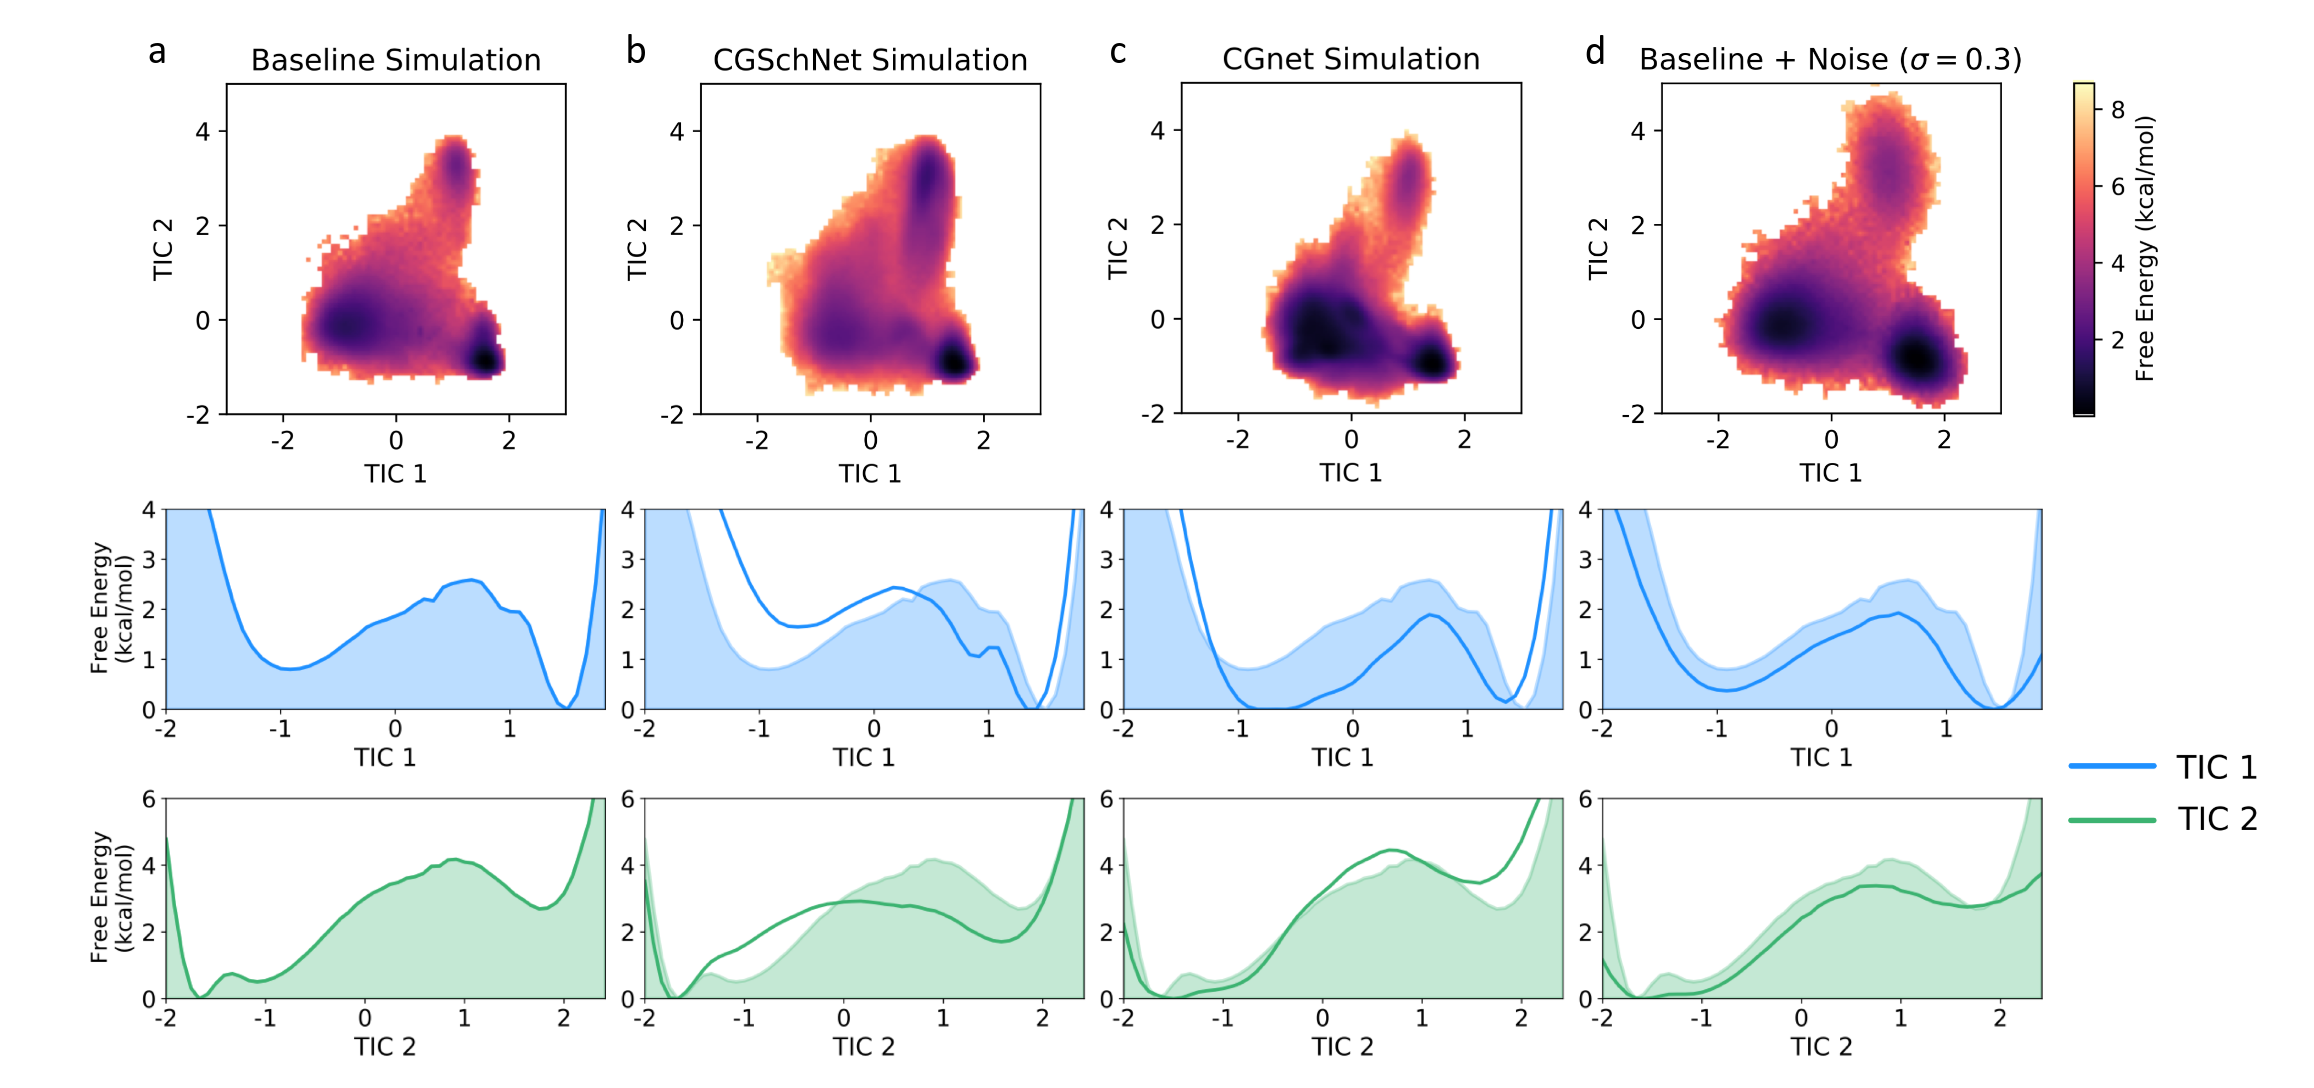
\includegraphics[width=0.8\linewidth]{./chignolin_results.png}
  \end{center}
\end{frame}
\begin{frame}
  \frametitle{Results (Chignolin)}
  \begin{center}
    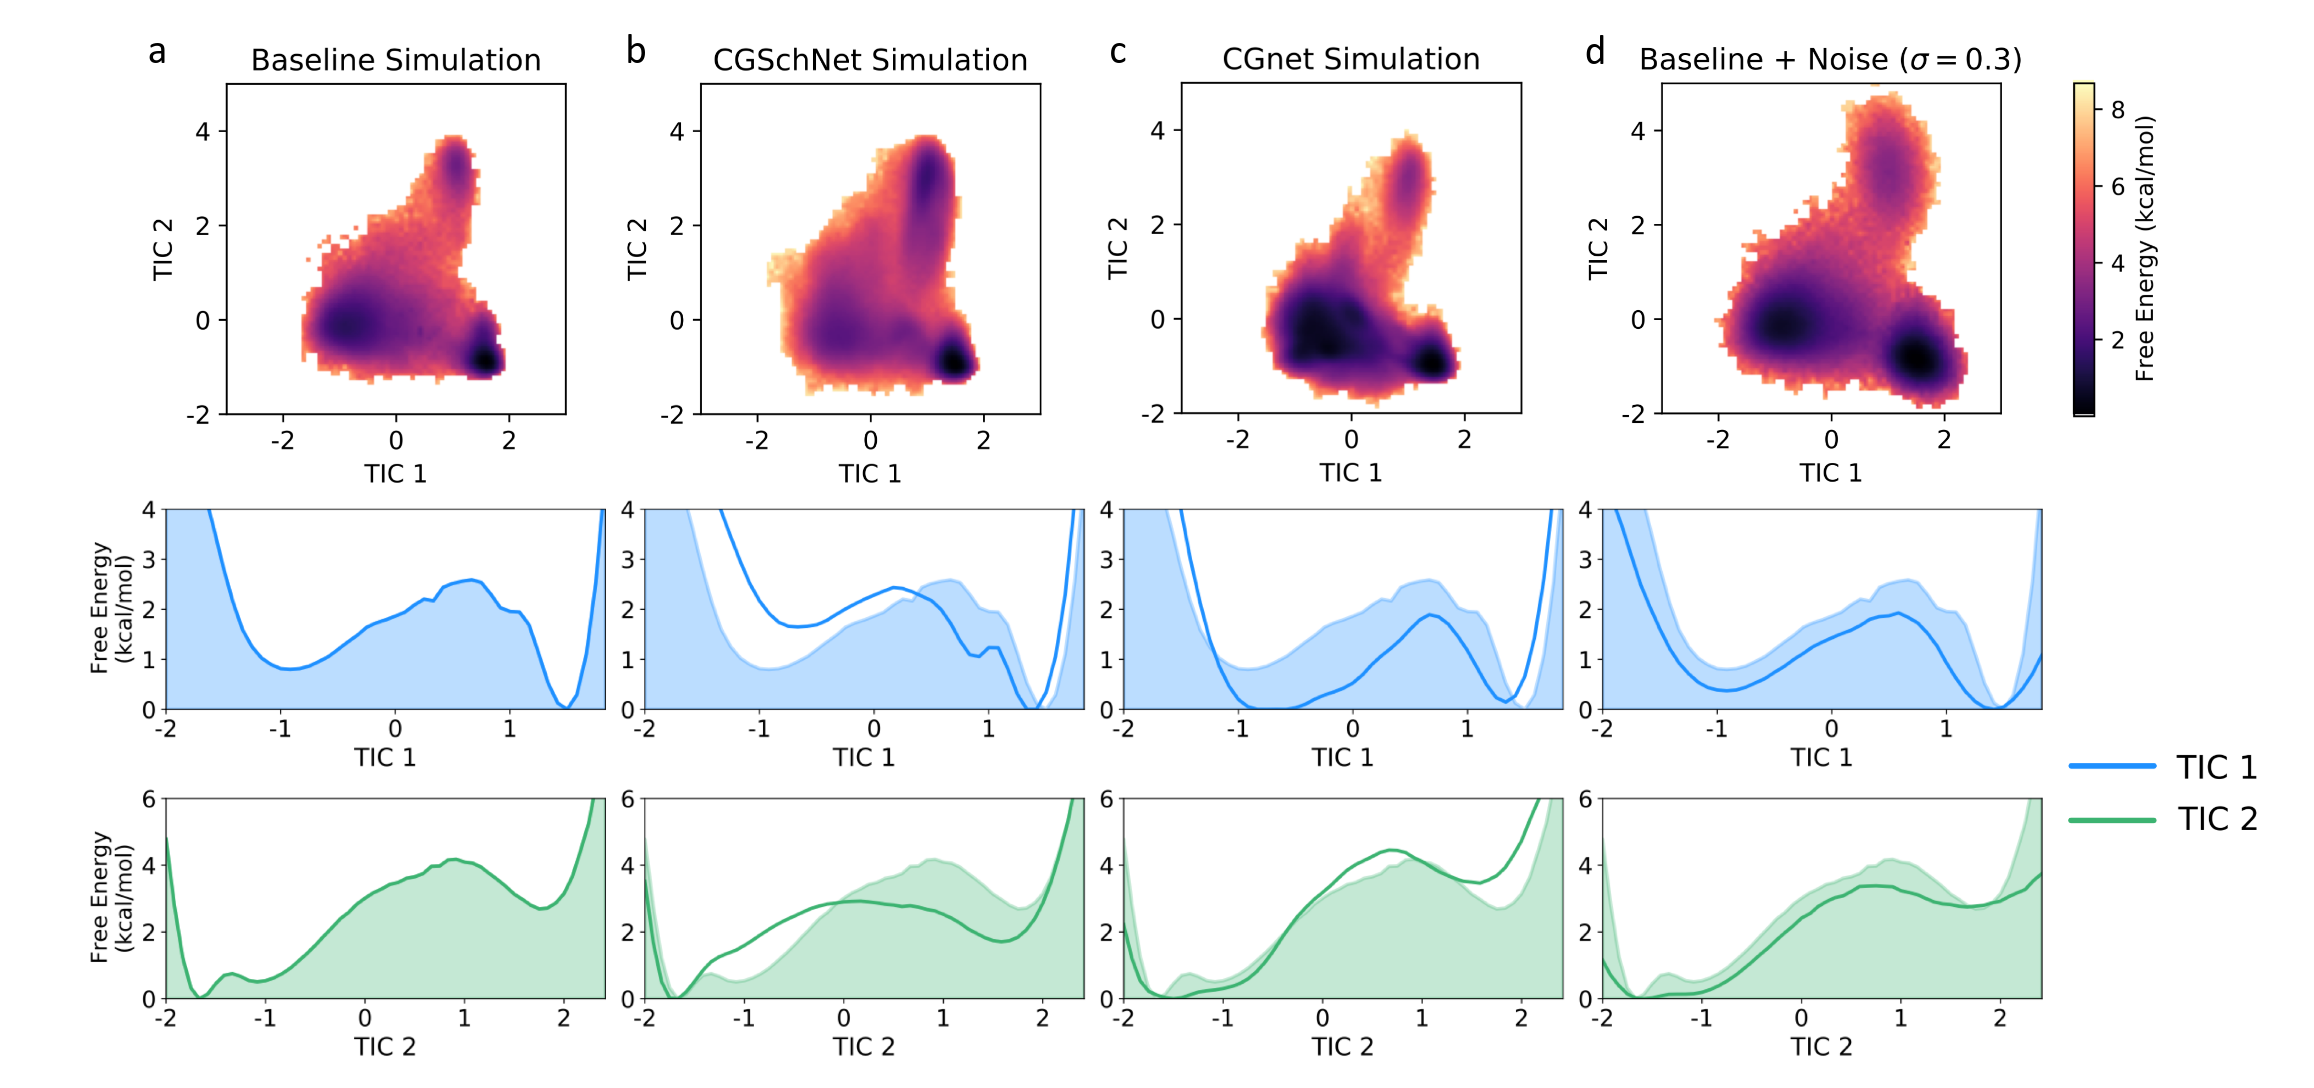
\includegraphics[width=0.6\linewidth]{./chignolin_results.png}
    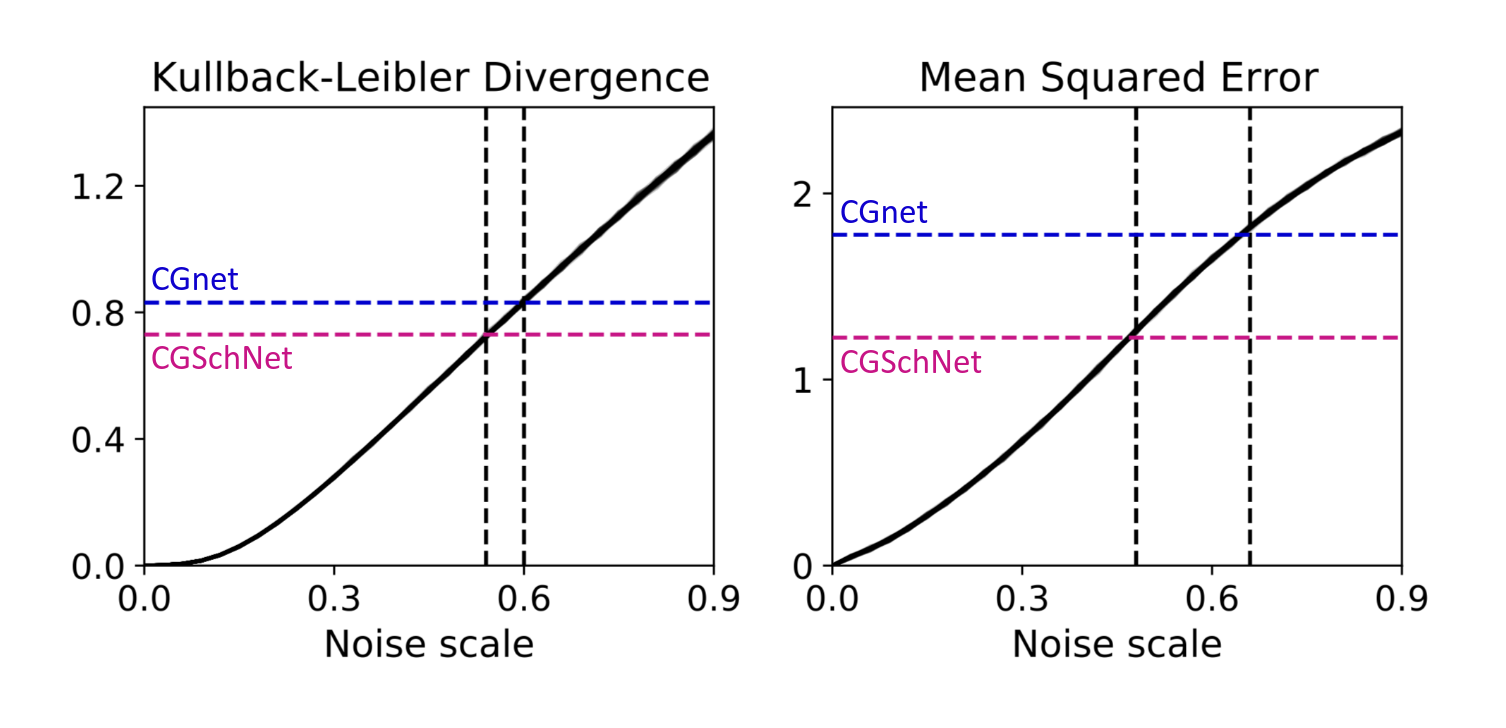
\includegraphics[width=0.6\linewidth]{./chignolin_divergence.png}
  \end{center}
\end{frame}
\begin{frame}
  \frametitle{Results (Capped alanine)}
  \begin{center}
    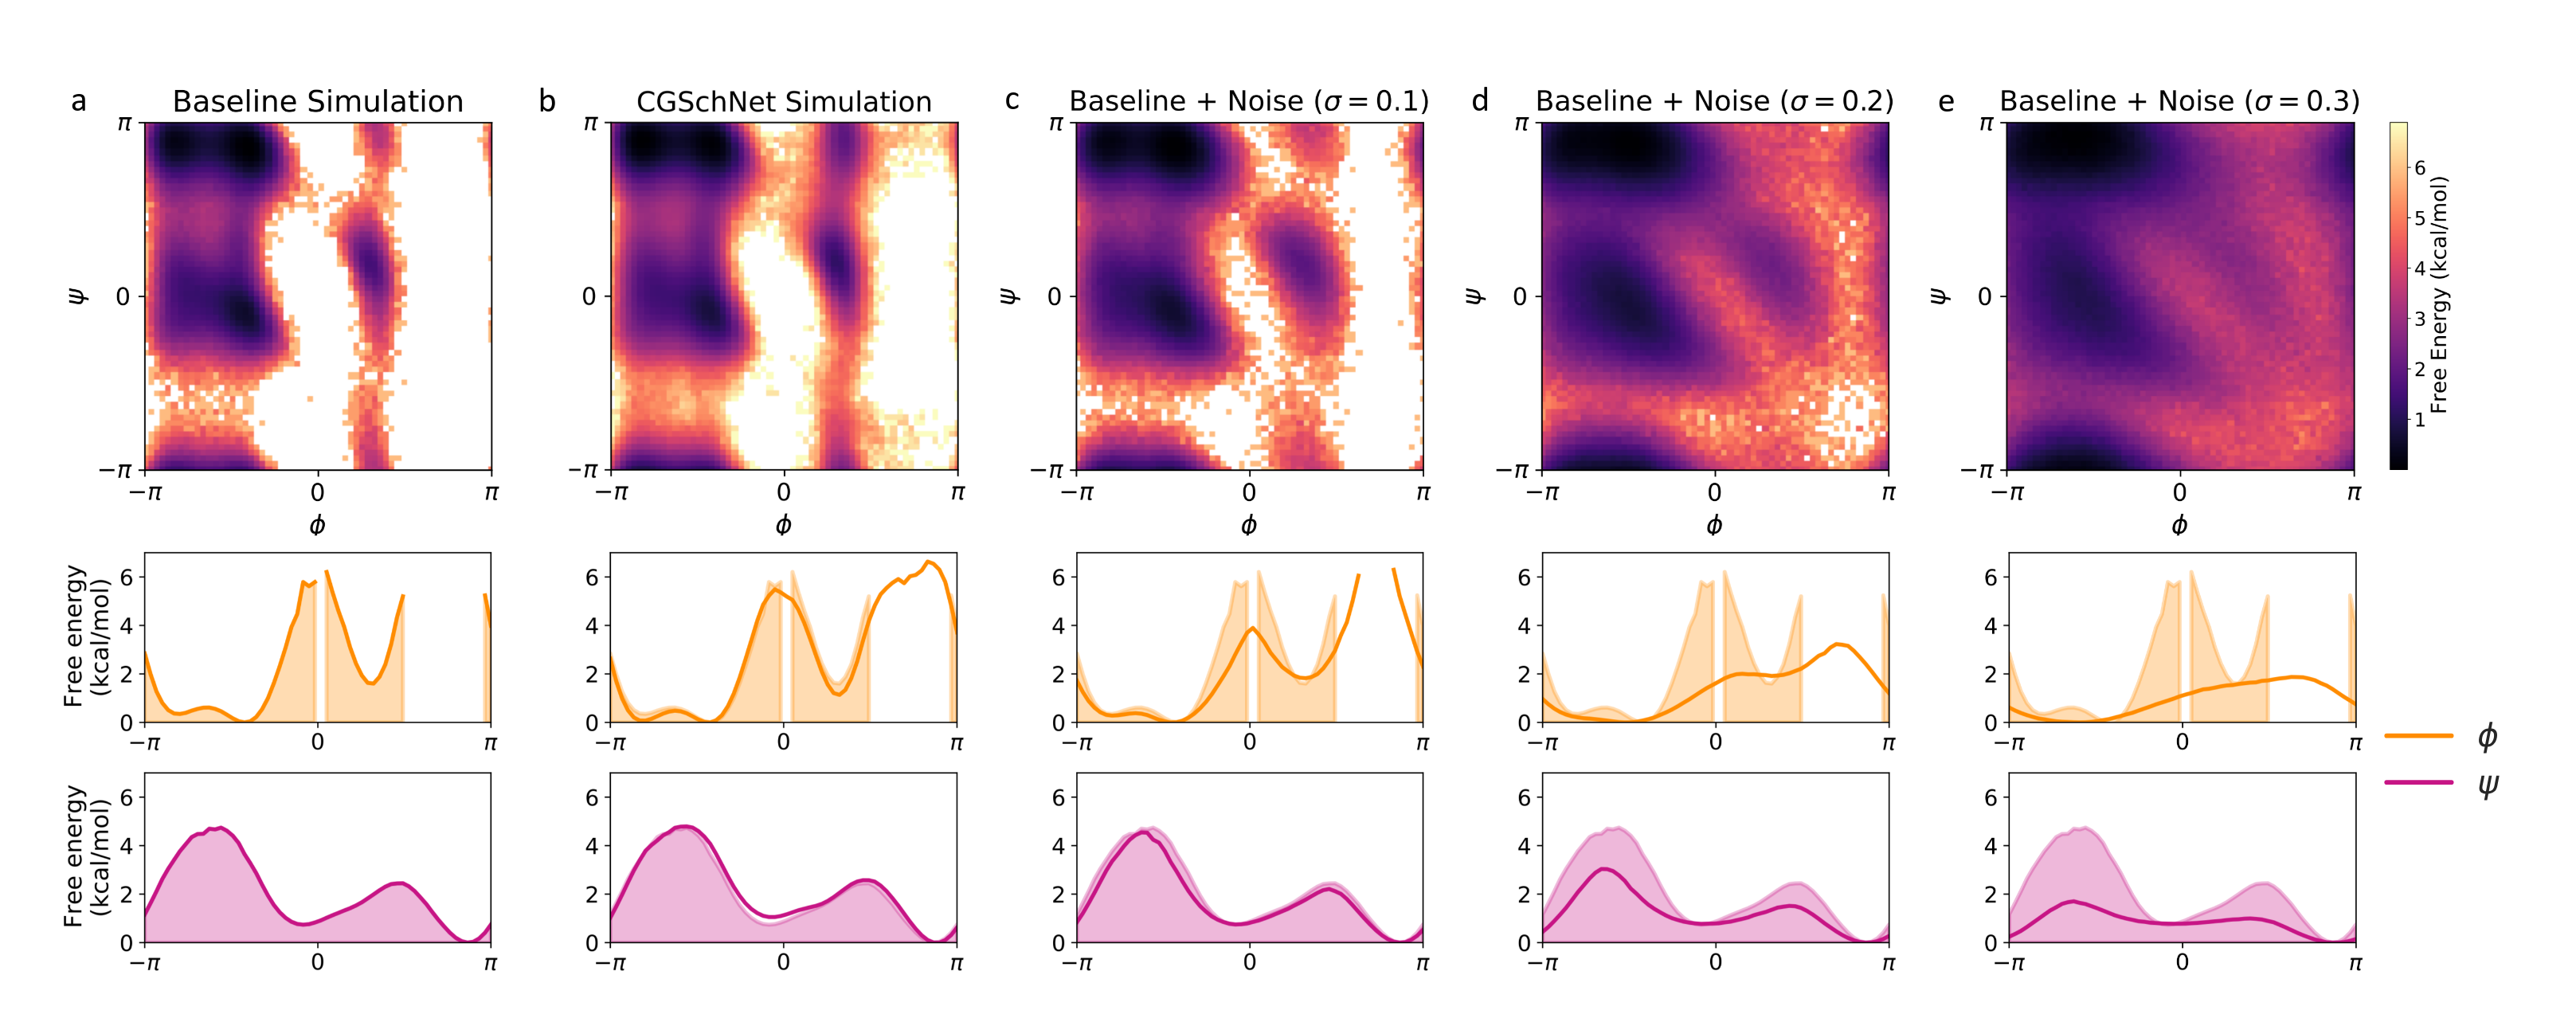
\includegraphics[width=0.6\linewidth]{./alanine_results.png}
    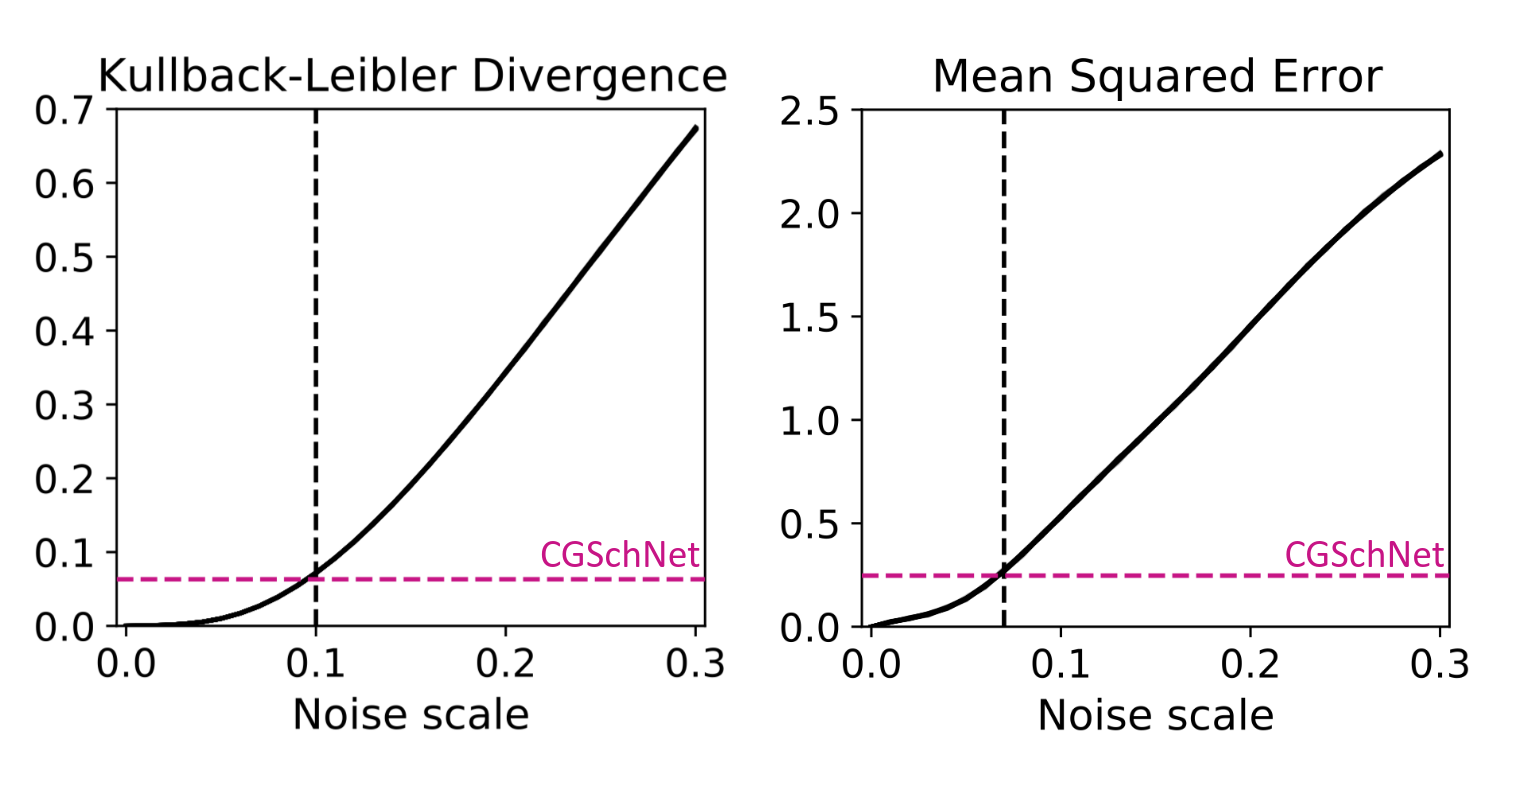
\includegraphics[width=0.6\linewidth]{./alanine_divergence.png}
  \end{center}
\end{frame}
\begin{frame}
  \begin{center}
    \Huge Q\&A
  \end{center}
\end{frame}
\end{document}
